
%\chapter{The effect of phenotypic plasticity on plant community dynamics}
%Hypothesis on the cumulative effect on niche and interactions.
%
%\section{Individual resistance and resilience against drought events}
%Amplitude and length of the event :\\
%- severity effect reduced by lower tau ?\\
%- resistance versus resilience: H0: conservative strategy have higher resistance, H1 : low tau allows for re-equilibrium and increase resistance (low amplitude and long length. H2: high tau allow to avoid dead-end situation during short severe drought (high resilience)
%\section{Community response to drought event}
%coexistence effect vs resistance/resilience effect\\
%uniform vs heterogenous (plasticity wise) community response
%H1: 
%

\begin{fullwidth}
This second result chapter examines the effects of phenotypic plasticity at the scale of the community. Another parameter filtering processes is performed and described in the first section of this chapter. The second part focuses of the effects of plasticity of the main properties of the community. The impact of plasticity on species diversity is particularly investigated. This chapter gives a glimpse of the potential of the model to answer various questions around the role of intraspecific variations on diverse community properties.
\end{fullwidth}

\chapter{Community level simulations: non plastic community}


\section{Parameter filtering}
\subsection{Method}

%\paragraph{Field data}
%Field data has been collected between years 201 .. and 201 by Claire Deleglise and al. (). Not used here.

\paragraph{Weather data}
Weather data for the time period between 1959 and 2014 has be computed by the MeteoFrance model SAFRAN by ... using GPS coordinates, slope, azimuth and horizon computed from a digital elevation model. These parameters were also used by the model CROCUS to compute snow accumulation and snow melting. These high frequency data (resolution under 1h) have been averaged on a daily time-step and used to compute input variables for \model. The snow in particular defines the length of the growing season starting with the first snow melt of the year and finishing the day of the first snow fall of autumn or winter.

The simulated years above 2014 are randomly sampled form the existing dataset between 1995 and 2014.

\paragraph{Parameter filtering}
Community level parameter filtering is conduced for a new table of parameter sets. These parameter sets are ... from accepted parameters and joined with LHS random sampling for five community level parameters: seed germination density, drought mortality, ageing mortality, plasticity cost for environmental sensing and plasticity cost for trait changes (see chapter \ref{chapter:model-description} for details).

Few words on why plasticity cost parameters: time limits, distinguish the benefit of plasticity itself, not combined effect. Should have done simulations with no cost to have an idea of plasticity cost effect. 

The simulations run over 300 hundreds years for 6 sites described in table \ref{table:sites} on squares of ... square centimetres. The simulation is stopped and the parameter set rejected if no individual persist and the seedbank is empty. The seedrain is composed of seeds contained in the seedbank and seeds from the metacommunity. The total of seeds is defined by the seed germination density and the area simulated. The seeds from the simulated community represent up to 80 \% of the seedrain, less if the seed production is limiting. The first ... years are not taken into account in the filtering process to let the community settle.


\paragraph{Simulations}

\subsection{Results}

Simulations done. Need to illustrate the results.\\

\paragraph{Effect of parameters}
On stability and on diversity (functional and species)\\
Random forest approaches like sensitivity analysis at individual scale.


\section{Non plastic communities}
Trade-off, diversity, stability ...


\paragraph{Ecological trade-off ?}
Is there a selection of some parameters ? Are there ecological trade-off (resource use strategy and reproduction) emerging from the model ?

\chapter{Plasticity: impact on species fitness and diversity}

Plasticity in integrated framework and full community simulations. Plasticity mechanisms, but also plasticity as a strategy (look at the cost and tau). 

Effects on productivity and coexistence. Difference in the correlation ?

Effect of tau on persistence.

\section{Plasticity and diversity}

Now 

\subsection{Method}

\paragraph{Simulations}
To test the effect of plasticity on coexistence and community dynamics, runs from the parameter filtering are used as starting points to limit the simulation time of the stabilisation phase. For each parameter set tested, 6 different sites were tested during the calibration phases, 77 parameter sets were accepted, resulting in 462 communities. Each of those is the starting point of three parallel runs that differ only by the allocation algorithm used: \textit{non plastic}, \textit{fixed-equilibrium} and \textit{plastic-optimisation}. The \textit{fixed-equilibrium} is favoured to \textit{fixed-optimisation} algorithm because previous part of the document focused on this algorithm and because it is simpler to analyse. The \textit{plastic-optimisation} algorithm is still simulated, despite the relatively poor performance results observed in constant conditions and the high convergence, because the introduction of plasticity cost, continuous species specific plasticity ($0 < \tau < 1$), and temporal and spatial heterogeneity should mitigate the negative sides of this allocation mechanism and give information of processes at stake.


\paragraph{Statistical tests}

The differences of effects between the different types of plasticity on the variables of interest are computed unpaired Wilcoxon tests assuming an independence of the the different data points. This assumption of statistical independence is justified by the normalisation for each parameter set of the variables relative to the mean of the \textit{non plastic} group. This normalisation allows to compare the simulations between the parameters sets. The interactions and other level (site, and autocorrelations) are discussed later in this section. 

\subsection{Results}

%Need to run the simulations. Script is almost ready, parameters are filtered from previous step.
%
%\paragraph{General behaviour} ?
%gradient along climatic gradient ? did I save the climate ? Nope, can't really say anything about it.

\paragraph{Effect on coexistence}


\begin{marginfigure}\label{fig:species_richness}
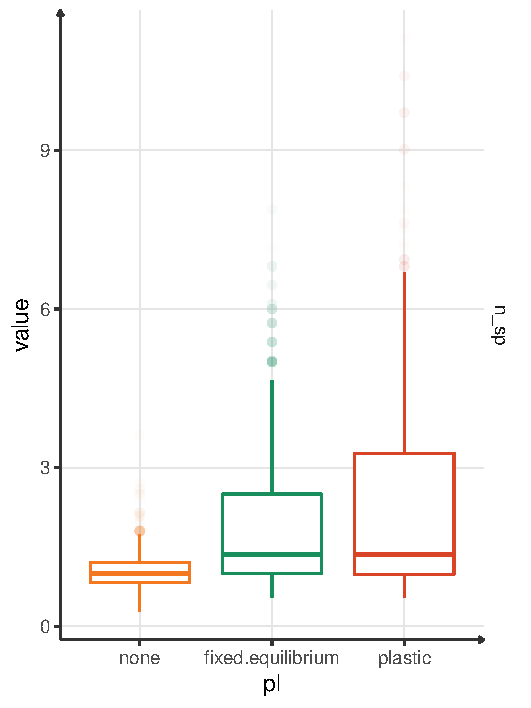
\includegraphics[]{./2_PP/Figures/Comm/comm_n_sp_differences.pdf}
\caption[Relative species richness in plasticity treatments]{Relative species richness in the three plasticity treatment. To negate the variability due to the parameter sets, the realised number of species is divided by the median number of species in \textit{non plastic} treatment for each parameter set. The variability is due to random invasion and climatic variability (inter-sites and inter-seasons).}
\end{marginfigure}

Plasticity is responsible for high portion of vairability, but also parameters: plasticity cost parameters:

\begin{figure}%[tb]
    \classiccaptionstyle
\sidebysidecaption{0.60\textwidth}{0.3\textwidth}{%
    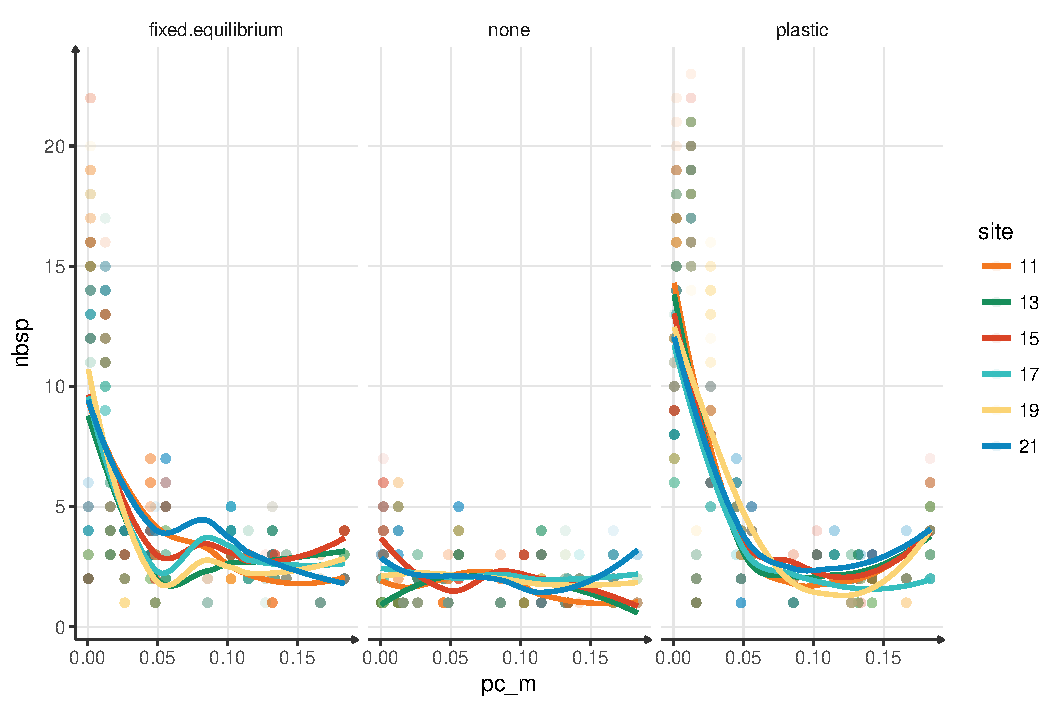
\includegraphics[width=1\linewidth]{./2_PP/Figures/Comm/comm_n_sp_pc_m.pdf}%
}{%
  \caption[Maintenance plasticity cost effect on species richness]{Effect of the cost of plasticity-maintenance on the absolute number of species in the three plasticity treatments. Individual season values (points) and site-specific trends (gam smoothing line) are represented.}
  \label{fg:pl_cost}
  }
\end{figure}

Consistent trends between sites. Inter-season variability (why didn't I save the weather?). Not super clean. Similar (but lower start for plastic distance diversity. Can be because of interactions %or because non variable enough.




%\paragraph{Plasticity selection}

%Not done yet. when is plasticity selected: is there a correlation between environment variables (or variations and plasticity selection). trade-off with other traits ?
\paragraph{Productivity}


\begin{marginfigure}\label{fig:total_BM_comm}
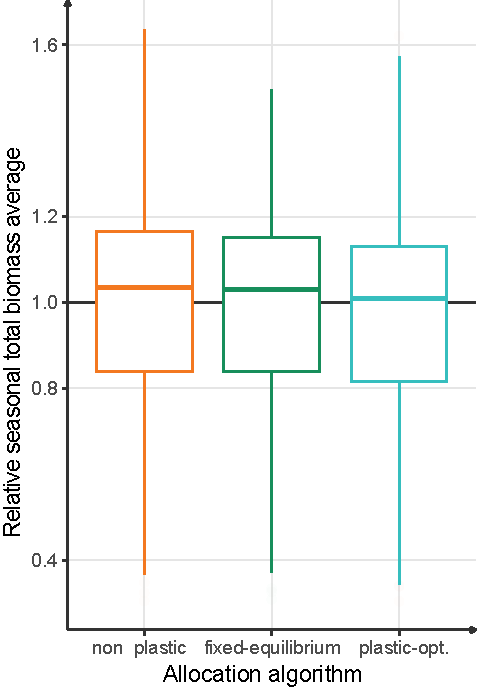
\includegraphics[width = \textwidth]{./2_PP/Figures/Comm/comm_BMtot_differences.pdf}
\caption[Plasticity levels in exclusive groups]{Plasticity levels of species that are present in only one type of plastic treatment.}
\end{marginfigure}

\paragraph{Community structure}

Becaue changes in community structure, no changes in density or productivity but, changes in structure, and competition evenness.

\begin{figure}%[tb]
    \classiccaptionstyle
\sidebysidecaption{0.60\textwidth}{0.3\textwidth}{%
    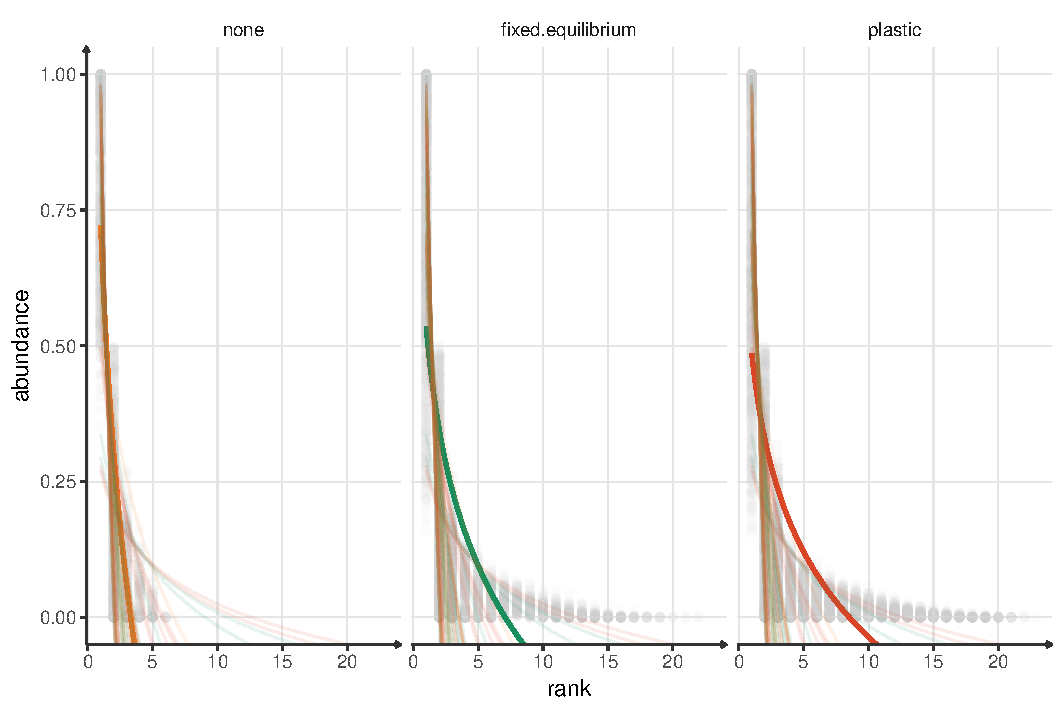
\includegraphics[width=1\linewidth]{./2_PP/Figures/Comm/comm_RAC_pl.pdf}%
}{%
  \caption[Rank-Abundance curves fits]{Rank-Abundance curves.}
  \label{fg:PCA_calibration}
  }
\end{figure}



\paragraph{Plasticity: a winning strategy ?}
Are plastic species more selected than the other ? Probably a bell-shape curves


\begin{marginfigure}\label{fig:tau}
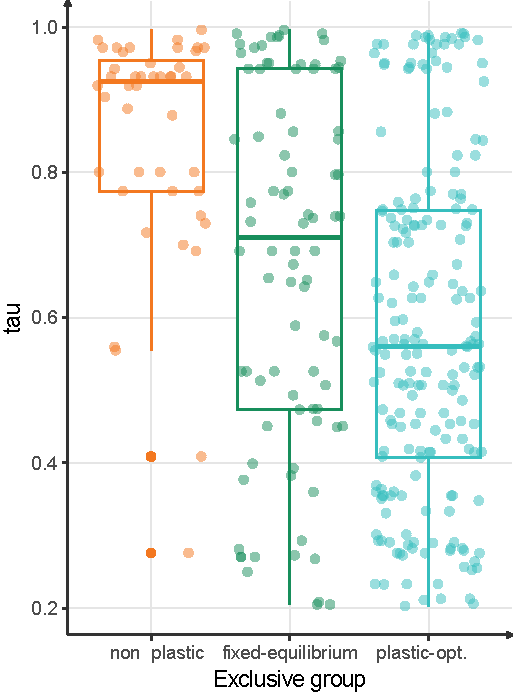
\includegraphics[]{./2_PP/Figures/Comm/comm_tau_differences_exclusive_groups.pdf}
\caption[Plasticity levels in exclusive groups]{Plasticity levels of species that are present in only one type of plastic treatment.}
\end{marginfigure}


%\section{Strategy}

%\subsection{Results}
\paragraph{Variable strats}

Select different strat? meh, from very site specific strats (one dominant species), to more variable within the site, but less differences between the strats. Shift from beta diversity to alpha diversity.

%Lead to changes in strats? If yes, is it direction\\
%al, or is the direction depends on species?%
%Do species change a lot there strategies?

%Is it always in the same direction for all species ? (reproduce Kichenin).

\subsection{Discussion}
\paragraph{Competition evenness}

Plasticity allows the emergence of new phenotypes that are plastic. Leading to higher density in competitors, and greater evenness. Hard to detect because not the same number of species, or require other experiments. 

\paragraph{shift in strategy}


also, Jung \cite{jung_intraspecific_2014} show contrasting response between species and within species - might not be the best 

\paragraph{Why higher diversity}

Plasticity allows for bigger niche (variability dimension), more chance to build enough "growth potential" to persist. Otherwise, other species that are dominant, because other species can settle, take advantage of it.
Should look at the growth rates hierarchy for a couple of simulations.


\paragraph{Independence of points}

Interaction between plasticity effects and parameter sets, but the interest here, even if  it is interesting. Higher variance due to site and weather. The almost perfect knowledge of models allows an extremely precise decomposition of the effects, but at the risks of loosing broad effects. The difficulty is to measure the relative strength of these effects, and generalise. But, by essence, the parameters are suspected to have a significant effect that can be identified, otherwise it would not have been included in the model.